\documentclass[twoside]{supsistudent} 

\usepackage{float}

% per settare noindent
\setlength{\parindent}{0pt}

% Crea un capitolo senza numerazione che pero` appare nell'indice %
\newcommand{\problemchapter}[1]{%
  \chapter*{#1}%
  \addcontentsline{toc}{chapter}{#1}%
\markboth{#1}{#1}
}

% Numerazione delle appendici secondo norma
\addto\appendix{
\renewcommand{\thesection}{\Alph{chapter}.\arabic{section}}
\renewcommand{\thesubsection}{\thesection.\arabic{subsection}}}

\setcounter{secnumdepth}{5} 	%per avere più livelli nei titoli
\setcounter{tocdepth}{5}		%per avere più livelli nell'indice

\titolo{XR Bridge: un wrapper OpenXR-OpenGL per applicazioni VR}
\studente{Lorenzo Adam Piazza}
\relatore{Peternier Achille}
\correlatore{-}
\committente{Peternier Achille}
\corso{Ingegneria informatica (Informatica TP)}
\modulo{C10826}
\anno{2023 / 2024}

\begin{document}

\pagenumbering{alph}
\maketitle
\onehalfspacing
\frontmatter

\pagenumbering{roman}
\tableofcontents
\listoffigures					% Opzionale
\listoftables					% Opzionale

\newpage
\mainmatter
\pagenumbering{arabic}
\setcounter{page}{1}

\chapter{Introduzione}

Lo scopo del progetto è sviluppare un wrapper (d'ora in poi chiamato XrBridge) attorno a OpenXR per permettere di sviluppare applicazioni che fanno uso di realtà virtuale e OpenGL in modo più semplice. XrBridge andrà a sostituire OvVR, un'implementazione simile già esistente sviluppata dal docente responsabile che fa uso di OpenVR. Dal momento che XrBridge verrà utilizzato nel corso di realtà virtuale (successore del corso di grafica), esso dovrà essere il più simile a OvVR possibile.

Aver personalmente seguito sia il corso obligatorio di grafica e il corso opzionale di realtà virtuale mi ha permesso di meglio capire i requisiti del progetto, sia dal punto di vista del docente che dovrà lavorare con XrBridge durante il suo corso, sia dal punto di vista dello studente che dovrà sviluppare un progetto che verrà poi valutato facendo uso di XrBridge.

L'aspetto più importante di XrBridge (oltre al fatto che deve funzionare) è la semplicità. Una soluzione troppo complessa sarebbe un problema sia per il docente, sia per lo studente. Una soluzione troppo complessa forzerebbe il docente a dedicare più tempo a spiegare agli studenti come funziona e come si utilizza XrBridge; il corso, infatti, è dedicato alla realtà virtuale, non a XrBridge. Tale soluzione causerebbe troppe difficoltà per gli studenti, poiché aggiungerebbe ancora più materiale da studiare e comprendere. Per sviluppare XrBridge è dunque molto importante sempre considerare il contesto in cui esso verrà utilizzato.

Lo scopo del corso di realtà virtuale è sviluppare un'applicazione in C++ che fa uso di realtà virtuale senza utilizzare game engines interagendo direttamente con API di basso livello come OpenGL e OpenVR. Il corso opzionale di realtà virtuale si basa sul corso obligatorio di grafica, dove lo scopo è sviluppare un'applicazione grafica 3D (ad esempio un piccolo gioco) senza fare affidamento a game engines esistenti o strumenti simili. Gli studenti imparano ad utilizzare OpenGL e a sviluppare personalmente un game engine che dovranno poi utilizzare per sviluppare l'applicazione grafica. Il corso di realtà virtuale consiste, in poche parole, ad estendere l'applicazione grafica sviluppata nel corso di grafica per aggiungere la funzionalità di realtà virtuale.

% TODO: Link to tutorial and doc
Questo documento non si tratta di una guida dettagliata a OpenXR e saranno spiegati solamente i concetti principali essenziali per comprendere questo progetto. Per più informazioni su OpenXR, fare riferimento al tutorial e alla documentazioni.

Inoltre, questo documento non spiega nel dettaglio ogni riga di codice presente all'interno del progetto, bensì può essere usato come accompagnamento. I dettagli di implementazioni sono visibili nel codice e commentati in modo approfondito.

% TODO: Explain why the teacher wants to replace OpenVR with OpenXR

\section{Pianificazione}

Di seguito sono descritte tutte le fasi svolte per sviluppare il progetto. Avere un piano che non sia troppo dettagliato ma allo stesso tempo completo ha garantito molta flessibilità nello sviluppo e ha permesso di sempre avere in vista l'obiettivo e rispondere facilmente ai vari problemi che sono stati incontrati durante lo svolgimento del progetto.

% TODO

\begin{enumerate}
  \item Analizzare l'approccio con la soluzione corrente già esistente di OvVR.
  \item \textbf{Applicazione demo OpenXR}: Sviluppare un'applicazione semplice per comprendere il funzionamento e la struttura di OpenXR. Questa applicazione permetterà all'utente di utilizzare un visore di realtà virtuale e visualizzare un semplice cubo e sarà interamente contenuta in un singolo file. Per sviluppare questa applicazione è stato seguito il tutorial ufficiale di OpenXR.
  \item \textbf{Definire struttura API}: Definire la struttura della API di XrBridge: inizializzazione, rendering, de-inizializzazione.
  \item \textbf{Cleanup} Separare il codice specifico dell'applicazione di prova dal codice generico di OpenXR e spostare quet'ultimo in un file separato che diventerà poi la libreria XrBridge.
  \item \textbf{Error handling}: Definire e implementare una gestione degli errori che sia semplice, intuitiva e funzionante.
  \item \textbf{Logging}: Migliorare i messaggi output di XrBridge per permettere all'utente di meglio comprendere cosa sta succedendo dietro le quinte.
  \item \textbf{Discutere con docente}: A questo punto si è discusso con il docente responsabile la qualità della soluzione sviluppata e quanto sia adatta al corso di realtà virtuale. Sono inoltre stati discussi parametri di default e altre opzioni per XrBridge. È molto importante che il docente dia feedback, poichè XrBridge dovrà essere utilizzato nelle lezioni del corso di realtà virtuale dal docente e dagli studenti.
  \item \textbf{Linux}: La maggior parte dello sviluppo fino a questo punto è avvenuto su Windows ed è ora il momento di implementare il supporto per Linux.
  \item \textbf{Documentazione API}: Una volta che la API di XrBridge è diventata stabile e finale, è stata scritta la documentazione utilizzando Doxygen.
  \item \textbf{Test}: Infine sono stati eseguiti dei test per determinare se la soluzione prodotta soddisfi i requisiti e funzioni correttamente in risposta a vari scenari.
\end{enumerate}

Questo rapporto è stato scritto durante tutte le fasi del progetto.

\section{Requisiti}

\begin{table}[H]
  \caption{Requisiti del progetto}
  \begin{center}
    \begin{tabular}{ | m{1cm} | m{6cm} | m{6cm} | }
      \hline
      ID   & Descrizione & Note \\
      \hline
      R-01 & XrBridge deve supportare la API grafica OpenGL & - \\
      \hline
      R-02 & XrBridge deve supportare la piattaforma Linux & - \\
      \hline
      R-03 & XrBridge deve supportare la piattaforma Windows & - \\
      \hline
      R-04 & XrBridge deve supportare la runtime SteamVR & - \\
      \hline
      R-05 & XrBridge deve supportare OpenXR versione 1.1 & - \\
      \hline
      R-06 & La API di XrBridge deve essere chiara e semplice & Il più simile possibile a OvVR. \\
      \hline
      R-07 & XrBridge deve essere utilizzabile con C++ & Il corso di realtà virtuale si svolge utilizzando C++. \\
      \hline
      R-08 & XrBridge deve supportare head-mounted-displays & Visori di realtà virtuale da indossare oppure uno smartphone. Durante il corso di realtà virtuale si usa lo smartphone. \\
      \hline
      R-09 & La API deve permettere all'utente di reperire posizione e rotazione del visore & - \\
      \hline
      R-10 & La API deve permettere di rilevare l'input dall'utente & - \\
      \hline
      R-11 & XrBridge deve supportare la libreria grafica FreeGLUT & L'uso di FreeGLUT è richiesto dai corsi di grafica e realtà virtuale. \\
      \hline
    \end{tabular}
  \end{center}
\end{table}

\chapter{Stato dell'arte}

Grazie all'evoluzione della tecnologia hardware e software nel corso degli ultimi decenni, è diventato sempre più facile sviluppare applicazioni di realtà virtuale di qualità sempre maggiore e sempre più immersive. È facile riconoscere questo progresso; basta confrontare le prime esperienze di realtà virtuale, come il Nintendo Virtual Boy, e confrontarle con i videogiochi VR di ultima generazione. Nel corso del tempo sono nati una moltitudine di strumenti per facilitare lo sviluppo di applicazioni VR, da hardware facilmente accessibile a utenti casalinghi a programmi che permettono di creare scenari immersivi trascinando con il mouse oggetti in una scena virtuale.

Ci sono diversi metodi e strumenti per sviluppare applicazioni VR; di seguito ne elencherò alcuni e descriverò in che modo XrBridge si differenzierà dalle soluzioni già esistenti. Alcuni di questi strumenti sono già utilizzati nel corso di realtà virtuale.

\section{Game engines}

Nella maggior parte dei casi, appoggiarsi su di un game engine già esistente è la scelta migliore, semplice e diretta per sviluppare un'applicazione di realtà virtuale. Un game engine permette di concentrarsi interamente sul contenuto dell'applicazione senza dover pensare a tutti i detagli necessari per avere un'applicazione grafica funzionante. Alcuni dei game engines più conosciuti che supportano lo sviluppo di applicazioni VR sono Unity, Unreal Engine e Godot.

Ci sono però alcuni scenari dove potrebbe essere necessario sviluppare un engine da zero; è il caso di un'applicazione con bisogni molto specifici non coperti da un engine già esistenti oppure, come in questo caso, se l'obiettivo è imparare a sviluppare un'applicazione partendo dalle basi. In questi casi, è necessario imparare ad utilizzari strumenti a livelli più bassi; le prossime sezioni sono dedicate ad alcuni di questi strumenti.

\section{OpenVR}

OpenVR si tratta di un SDK e API sviluppati da Valve per facilitare lo sviluppo do applicazioni VR. OpenVR è progettato per essere semplice da usare e si concentra principalmente su applicazioni per Head Mounted Displays (classici visori a occhiali). Per questo motivo, OpenVR è più limitato a confronto con OpenXR.

\section{OpenXR}

OpenXR si tratta di uno standard aperto creato da Khronos (lo stesso gruppo che ha sviluppato OpenGL e Vulkan) con lo scopo di sviluppare applicazioni che fanno uso di realtà virutale e realtà aumentata. La prima versione completa (versione 1.0) è stata rilasciata nel 2019 con lo scopo di risolvere la frammentazione che esiste attualmente nel mondo della realtà virtuale. A differenza di OpenVR, OpenXR è solamente uno standard che descrive una API e non offre nessun software già pronto ed è compito di produttori di hardware o piattaforme di sviluppare i software che implementano la API. Questi software vengono chiamati \textit{runtime}. Il vantaggio di avere una API standard è quello di permettere di sviluppare applicazioni che possono essere eseguite su una moltitudine di dispositivi. OpenXR è progettato per supportare moltissimi possibili scenari, dalla realtà aumentata, alla realtà virtuale utilizzando un headset ad un sistema cave. Questa flessibilità però viene al prezzo di una maggiore complessità rispetto a OpenVR.

\section{SteamVR}

SteamVR si tratta di un software sviluppato da Valve e distribuito attraverso la piattaforma Steam. SteamVR supporta Windows e Linux. SteamVR funge sia da implementazione di OpenVR, sia come runtime di OpenXR. Tutti i videogiochi che fanno uso di realtà virtuale distribuiti attraverso Steam fanno uso di SteamVR.

\section{OvVR}

OvVR è una libreria che funge da wrapper attorno a OpenVR sviluppata dal docente responsabile ed ha lo scopo di semplificare lo sviluppo di applicazioni VR per il corso di realtà virtuale. XrBridge andrà a sostituire questa libreria. OvVR è scritto in C++ ed è interamente contenuto in un singolo file header.

\chapter{Design e implementazione}

\section{API}

Di seguito è riportato il flusso di esecuzione di XrBridge:

\begin{figure}[h]
  \caption{Flusso di esecuzione di XrBridge}
  \centering
  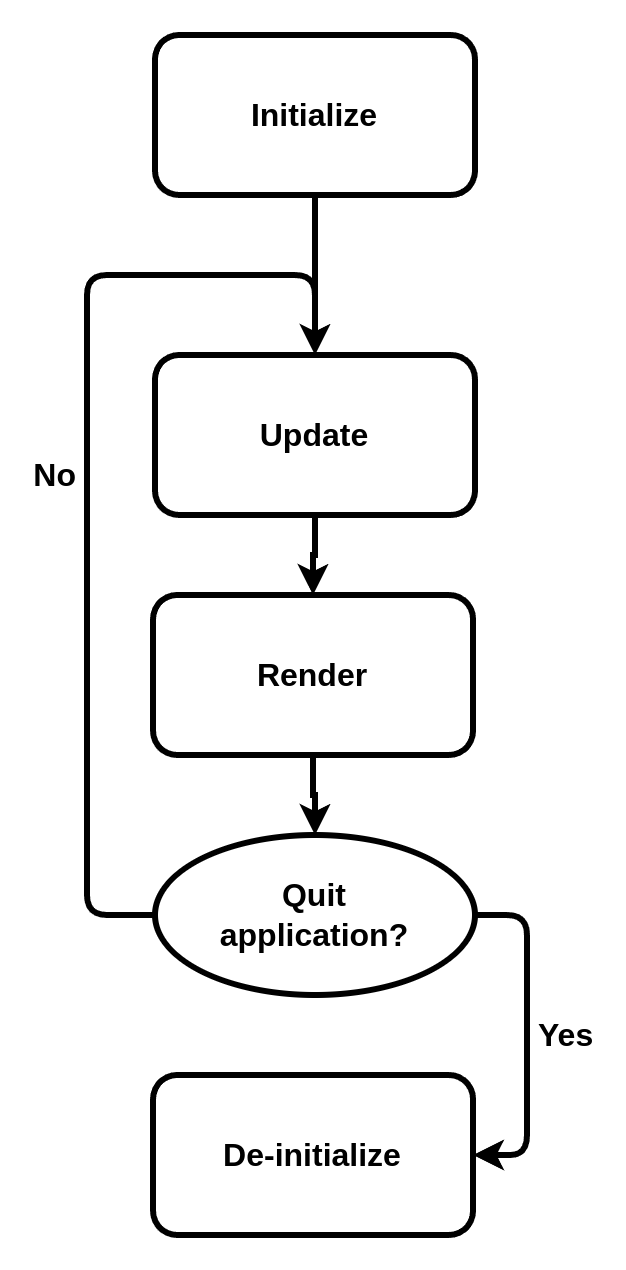
\includegraphics[scale=0.2]{resources/flow.png}
\end{figure}

Lo schema riporta le operazioni fondamentali necessarie per sviluppare un'applicazione grafica.

Uno degli aspetti più importanti della API è la semplicità. È importante che l'utente che farà uso di XrBridge si possa concentrare il più possibile sullo sviluppare la propria applicazione invece di dover pensare ai dettagli di implementazione della libreria. Questo significa che la API deve esporre solamente metodi e parametri che sono assolutamente necessari per l'utente e null'altro. Per questo motivo, è stato scelto di avere un metodo per ogni operazione fondamentale: inizializzazione, aggiornamento dello stato, render e de-inizializzazione. In realtà, aggiornamento e render potrebbero essere raggruppati in un'unica operazione, ma è stato deciso di lasciarli separati (se l'applicazione è in pausa e perciò non deve mostrare nulla, ma deve comunque rimanere in ascolto di eventi?). I dettagli della API e dei metodi si trovano nella documentazione apposita.

XrBridge è stato implementato sotto forma di una singola classe, dove ogni metodo pubblico rappresenta una delle operazioni fondamentali. Per facilitare l'utilizzo di XrBridge, oltre che ad offrire una documentazione più dettagliata della API e un'applicazione di essempio che ne dimostra chiaramente l'utilizzo, ogni metodo ha dei controlli per assicurarsi che essi vengono chiamati nell'ordine giusto (per esempio per assicurarsi che l'utente abbia inizializzato XrBridge prima di renderizzare una scena).

\subsection{Inizializzazione}

Il primo passo è quello di inizializzare XrBridge. Questo significa creare una connessione con la runtime di OpenXR, iniziare una sessione e caricare le estensioni necessarie. Questo passo è assolutamente necessario per poter utilizzare le funzionalità di OpenXR. Un errore durante questa fase è probabilmente causato da un problema con l'ambiente di esecuzione; potrebbe trattarsi di un errore di configurazione della runtime o un problema con l'hardware VR. Nessun'altra azione può essere eseguita prima dell'inizializzazione e l'inizializzazione può avvenire una sola volta (inizializzare più volte è considerato un errore).

XrBridge mette a disposizione il metodo \texttt{bool init(std::string\& application\_name)} per fare questo. Il parametro \texttt{application\_name} non è di molta importanza e viene utilizzato da SteamVR solamente come dettaglio visivo e non ha alcun effetto sull'esecuzione dell'applicazione. Per i dettagli sul suo utilizzo, fare riferimento alla documentazione sulla API e all'applicazione di esempio.

\subsection{Update}

Questa è una delle operazioni che vengono eseguite di continuo per la duranta dell'applicazione. Il metodo \texttt{bool update()} si occupa principalmente di gestire gli eventi generati da OpenXR, come ad esempio il termine di una sessione.

È inoltre importante per l'utente costantemente monitorare il valore di ritorno di questa funzione, poichè un errore potrebbe essere sollevato nel caso la runtime si disconnette (probabilmente l'utente ha disconnesso il suo visore o ha chiuso la runtime prima di terminare l'applicazione).

OpenXR fa distinzione fra un'istanza e una sessione. L'istanza è il collegamento alla runtime e viene creata una sola volta durante l'inizializzazione; mentre una sessione può essere terminata e ricreata più volte durante l'esecuzione dell'applicazione. Un'istanza viene generalmente terminata quando la runtime stessa viene terminata; in questo caso, XrBridge segnala un errore e necessita di un riavvio dell'applicazione. Nel caso che la sessione venisse terminata, invece, XrBridge attenderà semplicemente che la sessione venga ristabilita senza ritornare alcun errore o output.

\subsection{Render}

Questo è il passo più complesso di tutti e quello che differisce di più rispetto a OvVR. Come update, anche render viene seguito di continuo. Il rendering consiste nel generare le immagini che verranno poi proiettate sul visore VR seguendo le istruzioni dell'utente. L'utente invoca il metodo \texttt{bool render(render\_function\_t render\_function)} per renderizzare. L'argomento \texttt{render\_function} verrà spiegato più tardi.

OpenXR ha un sistema di rendering molto complesso che prende in considerazione la tempistica dei frame (refresh-rate), layers e swapchains.

OpenXR si aspetta che alcune azioni vengano eseguite entro un tempo limite stabilito dalla runtime. Nel caso il tempo limite scadesse, le conseguenze dipendono anche loro dalla runtime. Questo si applica anche al rendering dei frame. Nel caso di SteamVR, un mancato tempo limite potrebbe risultare in difetti grafici. Questa sincronizzazione è fatta dalla funzione \texttt{xrWaitFrame}.

Per costruire un frame, OpenXR utilizza un sistema di layers. Esistono diversi tipi di layers (3D, 2D, ...) che verranno poi sovrapposti (composizione) dalla runtime per generare l'immagine finale. È per esempio possibile avere un layer 2D dedicato alla GUI e un altro layer 3D per la scena. È anche posibilie utilizzare un singolo layer 3D e disegnare la GUI manualmente senza affidarsi alla composizione offerta da OpenXR. Questo è l'approccio di XrBridge, dove viene utilizzato un singolo layer di proiezione (layer 3D).

Il layer di proiezione si aspetta un certo numero di \textit{view}. Una view consiste in un'immagine che verrà mostrata sul dispositivo VR. Nel caso di un headset, ci saranno 2 view: una per l'occhio destro e una per l'occhio sinistro. È dunque necesario renderizzare la scena una volta per ogni occhio.

Una delle maggiori differenze tra OpenVR e OpenXR, quandi si tratta di rendering, è chi si occupa di generare i framebuffers che verranno utilizzati per il rendering. Nel caso  di OpenVR, è compito dell'utente creare i framebuffers, riempirli e inviarli a OpenVR una volta che il rendering è completo. Al contraro, OpenXR esige che sia la runtime a creare i framebuffers e che l'utente deve richiedere i framebuffers prima di poterli utilizzare. Questa differenza cambia in modo significativo la struttura dell'applicazione dal punto di vista del corso di realtà virtuale. Se prima gli studenti dovevano imparare il funzionamento per poter creare i propri framebuffers, ora questo processo è automatico.

Di seguito è riportata la sequenza di azioni richiete da OpenXR per renderizzare una scena. Le parti in italico sono implementate dall'utente, mentre il resto è eseguito automaticamente da XrBridge.

\begin{enumerate}
  \item Attendere il momento giusto per inizare a renderizzare il frame (sincronizzazione).

  \item Preparare il rendering dell'intero frame (begin).

  \item Preparare il rendering dell'occhio \textbf{sinistro} (begin).
  \item \textit{Renderizzare la scena dalla propsettiva dell'occhio sinistro}.
  \item Finalizzare il rendering dell'occhio sinistro (end).

  \item Preparare il rendering dell'occhio \textbf{destro} (begin).
  \item \textit{Renderizzare la scena dalla propsettiva dell'occhio destro}.
  \item Finalizzare il rendering dell'occhio destro (end).

  \item Finalizzare il rendering dell'intero frame (end).
\end{enumerate}

Il frame è mostrato all'utente solamente alla fine di tutta la procedura di render, quando tutte le view sono complete.

Come si può notare, ci sono due sequenze di \textit{begin - ... - end}: una per l'intero frame e una per ogni view/occhio.

Una possibilità di implementazione consiste nell'avere un metodo per ogni fase (\textit{begin\_frame}, \textit{beign\_eye}, \textit{end\_eye}, \textit{end\_frame}). Questa soluzione ha alcuni problemi: 1) una grande quantità di metodi sarebbero richiesti; 2) questo richiederebbe che l'utente faccia molta attenzione che ogni metodo sia chiamato nell'ordine corretto; 3) questo approccio non è scalabile (se si volesse sviluppare un'applicazione con una sola view?); 4) non è un approccio elegante; 5) è complesso da implementare.

Per XrBridge è stato scelto un approccio che appare molto più pulito, ordinato, semplice e scalabile: l'utente fornisce una propria funzione di render che verrà invocata quante volte necessario da XrBridge. È possibile utilizzare una lambda per questo, come nell'esempio seguente (semplificato):

\begin{verbatim}
  void render()
  {
    // ...

    xrbridge.render([&] (
      Eye eye,
      shared_ptr<Fbo> fbo,
      mat4 proj_matrix,
      mat4 view_matrix,
      uint32_t width,
      uint32_t height)) {

        // Render scene

      });

      // ...
    }
\end{verbatim}

Per più dettagli sul metodo e gli argomenti, fare riferimento alla documentazione di XrBridge.

Lo svantaggio principale di queso approccio è il fatto che richiede conoscienza delle lambda, anche se minima.

Un grande vantaggio che si può notare dall'esempio è il fatto che, per ogni volta che la lambda viene chiamata, è facile reperire tutte le informazioni necessarie per renderizzare la scena: questo include il framebuffer da utilizzare, le matrici di proiezione e view e altri parametri che si possono aggiungere se desiderato senza necessitare di grandi modifiche al codice. Questo permette di semplificare la API ancora di più, dal momento che non sono necessari metodi appositi per recuperare queste informazioni. Ad ogni chiamata della lambda, tutte le informazioni necessarie sono subito a disposizione. Utilizzando la lista di cattura della lambda, catturando tutto come mostrato nell'esempio sopra, permette di eseguire operazioni di preparazione una sola volta (ad esempio costruire la lista di render) invece che sprecare risorse e ripetere le stesse operazioni per ogni chiamata della lambda. Se utilizzato in questo modo, dal punto di vista dell'utente, questo approccio diventa molto semplice da capire e implementare e permette di ignorare quasi completamente le complessità che nascono dall'utilizzo di lambda.

\subsection{De-inizializzazione}

Questo si tratta dell'ultimo passo, dopo il quale l'istanza di XrBridge diventerà inutilizzabile. A questo punto l'utente dovrà riavviare l'applicazione oppure creare una nuova istanza. Il metodo \texttt{bool free()} si occupa di terminare la sessione, l'istanza e liberare tutte le risorse utilizzate.

\subsection{Gestione errori}

Esistono svariati approcci alla gestione degli errori nel codice. I due approcci più puliti e ordinati sono \textit{exceptions} e \textit{errors as values}. Per questo progetto è stato scelto il secondo approccio, per alcuni motivi: 1) è lo stesso approccio utilizzato da OvVR; 2) è lo stesso approccio utilizzato da OpenXR; 3) è più semplice rispetto alle eccezioni; 4) nessuna interruzione inaspettata del flusso di esecuzione.

Tutti i metodi di di XrBridge seguono quindi la stessa convenzione: ritornano un valore \texttt{true} se il metodo è stato eseguito con successo e \texttt{false} in caso di errore. Inoltre, in caso di un errore, un messaggio che descrive l'errore viene stampato su stderr.

\section{Strumenti e linguaggi di programmazione}

Dal momento che XrBridge andrà a sostituire una libreria già in uso scritta in C++ e che i corsi di grafica e realtà virtuale fanno uso unicamente di C++, anche XrBridge verrà scritto in C++; nessun altro linguaggio di programmazione è necessario per la libreria.

Inoltre, nessuno strumento specifico è necessario per sviluppare la libreria. Ogni strumento aggiuntivo serve unicamente per sviluppare l'applicazione

\section{OpenXR}

\subsection{Documentazione}

OpenXR offre una documentazione molto estesa che descrive nei dettagli come la API deve essere utilizzata e come una runtime deve essere implementata. Ci sono due principali tipi di documentazione: un manuale mirato principalmente a chi desidera utilizzare OpenXR che spiega come fare uso della API OpenXR, e una specifica mirata a chi desidera implementare una runtime di OpenXR.

Il manuale della API è accessibile tramite il seguente link: https://registry.khronos.org/OpenXR/specs/< VERSIONE >/man/html/, dove VERSIONE è la versione di OpenXR che si sta utilizzando (Per esempio 1.0). Si può accedere velocemente al manuale di una funzione o struct specifica con un link del seguente formato: https://registry.khronos.org/OpenXR/specs/< VERSIONE >/man/html/< FUNZIONE O STRUCT >.html. Il manuale mostra informazioni come le definizione delle funzioni e i loro parametri, possibili errori e una descrizione dettagliata della funzionalità.

La specifica di OpenXR è invece accessibile tramite il seguente link: https://registry.khronos.org/OpenXR/specs/1.0/html/xrspec.html. Come già detto, questo è utile principalmente per chi desidera implementare una runtime e non chi a chi semplicemente desidera utilizzare la API per sviluppare un'applicazione VR. Per questo progetto, ho usato molto raramente il documento di specifica.

OpenXR offre inoltre un tutorial ufficiale che spiega come sviluppare una semplice applicazione VR facendo uso di OpenXR. Il tutorial è accessibile al seguente link: https://openxr-tutorial.com/ e permette di scegliere la combinazione di piattaforma e API grafica che si desidera utilizzare. Per questo progetto ho utilizzato Windows / OpenGL, dal momento che l'implementazione per Linux non differiva da quella di Windows. Ho seguito attentamente questo tutorial per comprendere il funzionamento di OpenXR e per sviluppare una semplice applicazione dalla quale ho poi estratto il codice necessario per sviluppare XrBridge.

\subsection{Versioni}

Al momento dello svolgimento di questo progetto, ci sono due versioni principali di OpenXR: 1.0 e 1.1. Le differenze principali tra queste due versioni sembrano minime e non importanti per questo progetto; ho scelto perciò di utilizzare la versione 1.0 per avere la massima compatiblità con le runtime.

Le principali differenze tra le due versioni sono due: sono stati apportati miglioramenti alla specifica di OpenXR e alcune estensioni sono state incluse in OpenXR core.

\subsection{Runtime}

OpenXR non si tratta di un software specifico, bensì di un'interfaccia standard di API che permette di sviluppare applicazioni di realtà aumentata per svariati dispositivi. Una runtime è semplicemente un software che implementa lo standard e offre alle applicazioni un'interfaccia con un dispositivo di realtà virtuale. È compito degli sviluppatori di dispositivi per realtà virtuale svilupare una runtime per il proprio dispositivo. I requisiti di questo progetto richiedono che XrBridge debba funzionare almeno con SteamVR (una runtime di OpenVR e OpenXR sviluppata da Valve); dal momento che OpenXR è uno standard, XrBridge dovrebbe funzionare con tutte le altre runtime che implementano lo standard OpenXR correttamente, salvo per piccoli aggiustamenti.

Per permettere alle applicazioni di trovare la runtime corretta installata sul computer dell'utente, ogni runtime fa uso di un file manifest, ovvero un file di formato JSON che contiene alcune informazioni basi come il nome della runtime e il suo percorso nel filesystem. Questi file manifest sono generalmente installati in percorsi standard predefiniti (definiti dallo standard OpenXR) che dipendono dalla piattaforme; in alternativa è possibile specificare un percorso non-standard attraverso una variabile d'ambiente.

% TODO: https://registry.khronos.org/OpenXR/specs/1.0/loader.html#runtime-manifest-file-format
% TODO: https://registry.khronos.org/OpenXR/specs/1.0/loader.html#active-runtime-information

\subsection{Loader}

OpenXR utilizza un loader, ovvero un programma che ha lo scopo di individuare una runtime di OpenXR sul computer dell'utente. Questo programma viene sotto forma di una libreria che viene inclusa in un'applicazione VR. All'avvio dell'applicazione il loader cerca un file manifest di una runtime valido (TODO: chapter Runtime), stabilisce una connessione con la runtime e carica tutte le funzioni relative a OpenXR (run-time linking). Questo funziona in modo simile a librerie come GLEW per OpenGL.

OpenXR non offre un loader già compilato ed è quindi necessario compilarlo manualmente. L'applicazione Test include la libreria del loader già compilata e pronta all'uso. La versione di questa libreria è la 1.1.37. Di seguito sono riportate le istruzioni di come compilare la libreria loader per Windows utilizzando Visual Studio 2019 (per i seguenti passi è necessario Python 3; su Linux è possibile installare il loader utilizzando il package manager della distribuzione):
% TODO: Format
1. Scaricare e decomprimere il codice sorgente dal seguente link: https://github.com/KhronosGroup/OpenXR-SDK/releases/tag/release-1.1.37 (è possibile scegliere un'altra versione; per questo progetto solo la versione 1.1.37 è stata verificata).
2. Creare la cartella `build/` nella root della repository.
3. Dall'interno di `build/`, creare il file di progetto di Visual Studio utilizzando cmake: \$ cmake -G 'Visual Studio 16 2019' -DDYNAMIC\_LOADER=ON .. . È possibile scegliere un'altra versione di Visual Studio.
4. Aprire la soluzione `OPENXR.sln` appena creata con Visual Studio.
5. Scegliere la configurazione desiderata; per questo progetto è stato utilizzato *Release* e *x64*.
6. Compilare il progetto openxr\_loader.
7. Recuperare i file generati dal percorso build/src/loader/Release. I file necessari sono openxr\_loader.dll e openxr\_loader.lib.

\subsection{Filosofia della API}

OpenXR segue una filosofia molto simile a Vulkan, essendo stato sviluppato dallo stesso gruppo. Ogni funzione di OpenXR è caratterizzata dal prefisso `xr` seguito dal nome della funzione in camel case. Il passaggio di parametri alle funzioni di OpenXR viene fatto attraverso uno struct, il quale contiene un campo per ogni argomento che la funzione accetta e ha il prefisso \texttt{Xr}. Ogni funzione accetta almeno uno struct, anche se non necessita di parametri. Questo causa alcuni scenari interessanti, dove una funzione accetta come parametro uno struct senza membri. Ogni struct ha almeno due membri: \texttt{type}, il quale deve essere assegnato al momento della creazione dello struct e il suo valore è definito dallo standard OpenXR e \texttt{next}, il quale si tratta di un puntatore ad un altro struct in modo da permettere di estendere uno strct creando una catena. Nella maggior parte dei casi il membro \texttt{next} avrà un valore di \texttt{nullptr}.

\begin{verbatim}
  // Inizializza tutti i campi dello struct al loro valore di default.
  XrInstanceCreateInfo instance_create_info = {};
  // Configura il tipo della struttura.
  instance_create_info.type = XR_TYPE_INSTANCE_CREATE_INFO;
  // Configura gli altri parametri ...
  instance_create_info.createFlags = NULL;
  // ...
\end{verbatim}

\subsection{Layers e estensioni}

Similmente a Vulkan, OpenXR permette di estendere le proprie funzionalità attraverso dei layers e delle estensioni.

Un layer, come suggerisce il nome, è uno strato che può essere inserito fra OpenXR e l'applicazione. Un layer può offrire funzionalità come ad esempio tracing delle chiamate delle funzioni. Per questo progetto, non è stato necessario nessun layer. In caso si voglia aggiungere un layer, è sufficiente aggiungere il suo nome alla riga seguente all'interno di \texttt{xrbridge.cpp}, nella funzione \texttt{init}:

\begin{verbatim}
  const std::vector<std::string> requested_api_layers = { };
\end{verbatim}

Le estensioni, invece, permettono di aggiungere funzionalità extra a OpenXR. Alcune estensioni sono sviluppate da Khronos, ma possono anche essere sviluppate da terze parti. Per questo progetto, una singola estensione è stata necessaria: \texttt{XR\_KHR\_opengl\_enable}. Come suggerisce il nome, questa estensione abilita il supporto per la API grafica OpenGL.In caso si voglia aggiungere un'altra estensione, è sufficiente aggiungere il suo nome alla riga seguente all'interno di \texttt{xrbridge.cpp}, nella funzione \texttt{init}:

\begin{verbatim}
  const std::vector<std::string> requested_extensions = {
    "XR_KHR_opengl_enable",
  };
\end{verbatim}

\subsection{Binding grafico}

OpenXR fa uso di "graphic bindings", ovvero strutture che legano assieme una API grafica e una piattaforma. All'interno del codice, questi binding sono implementati sotto forma di struct. Esiste uno struct per ogni combinazione di API grafica (OpenGL, Vulkan, DirectX, ...) e piattaforma (Win32, X11, Wayland, ...) supportate e ogni struct richiede dei parametri legati alla piattaforma e alla API grafica scelta. Questi struct sono definiti nel file \texttt{openxr\_platform.h} della libreria OpenXR. Ecco alcuni esempi:

\begin{table}[H]
  \caption{Strutture per il binding grafico}
  \begin{center}
    \begin{tabular}{ l l l }
      API grafica & Piattaforma & Nome struct \\
      \hline
      OpenGL      & Windows         & \texttt{XrGraphicsBindingOpenGLWin32KHR} \\
      OpenGL      & Linux (Xlib)    & \texttt{XrGraphicsBindingOpenGLXlibKHR} \\
      OpenGL      & Linux (Wayland) & \texttt{XrGraphicsBindingOpenGLWaylandKHR}
    \end{tabular}
  \end{center}
\end{table}

Durante l'inizializzazione di OpenXR, è compito dello sviluppatore istanziare e popolare uno di questi stuct per la piattaforma che so vuole utilizzare. I requisiri richiedono solamente il supporto per OpenGL su Windows e Linux. Di seguito sono descritti gli approcci all'implementazione dei binding richiesti.

\subsubsection{Binding OpenGL + Windows}

Il binding OpenGL + Windows è rappresentato dalla struttura (\texttt{XrGraphicsBindingOpenGLWin32KHR}. Di seguito è riportata la definizione dello struct (i parametri \texttt{type} e \texttt{next} non sono importanti per questo capitolo):

\begin{verbatim}
  typedef struct XrGraphicsBindingOpenGLWin32KHR {
    XrStructureType             type;
    const void* XR_MAY_ALIAS    next;
    HDC                         hDC;
    HGLRC                       hGLRC;
  } XrGraphicsBindingOpenGLWin32KHR;
\end{verbatim}

I due parametri importanti sono \texttt{hDC} e \texttt{hGLRC} e fanno parte della API Win32. \texttt{hDC} si tratta del \textit{device context}, mentre \textit{hGLRC} è il \textit{OpenGL Rendering Context}; non è importante cosa rappresentato questi parametri, ma è necessario averli.

Qui si incontra un ostacolo: il contesto di OpenGL viene generato automaticamente da FreeGLUT. Per questioni di portabilità, FreeGLUT non offre un modo di recuperare questi parametri; a noi servono gli stessi parametri che FreeGLUT ha usato per creare il contesto OpenGL, il che significa che non possiamo generare un nuovo contesto/generare nuovi parametri. Fortunatamente, la API Win32 di Windows offre un modo per recuperare entrambi i parametri grazie alle funzioni \texttt{wglGetCurrentDC} e \texttt{wglGetCurrentContext} - queste due funzioni non accettano parametri. Grazie a queste funzioni, è possibile popolare tutta la struct e, di conseguenza, configurare OpenXR per questa piattaforma.

\subsubsection{Binding OpenGL + Linux}

Questo binding è più complesso rispetto a quello di OpenGL + Windows per due motivi.

La prima complicazione è dovuta al fatto che Linux non ha una API standard per quanto riguarda gli ambienti grafici. Al momento esistono infatti due principali piattaforme grafiche su Linux: X11 e Wayland. Inoltre, per X11, esistono approcci diversi per ognuna delle due librerie X11 più diffuse: Xcb e libX. Per questo motivo, esistono 3 struct per il binding OpenGL + Linux: \texttt{XrGraphicsBindingOpenGLXlibKHR} (LibX), \texttt{XrGraphicsBindingOpenGLXcbKHR} (Xcb) e \texttt{XrGraphicsBindingOpenGLWaylandKHR} (Wayland).

Inizialmente avevo deciso di utilizzare Wayland per due motivi. Il primo motivo è che lo struct per questo binding richiede un solo parametro, probabilmente rendendo più semplice l'implementazione. Il secondo motivo è il fatto che Wayland sta andando sempre di più a sostituire X11, tanto che molte delle distribuzioni di Linux principali supportano Wayland out-of-the-box. Lo svantaggio è il fatto che non è possibile eseguire applicazioni Wayland su X11. Questo approccio non è stato possibile a causa dell'assenza di supporto per Wayland in FreeGLUT. Nonostante FreeGLUT abbia un'implementazione di Wayland, come anche suggerito da un commento di uno degli sviluppatori (TODO: link to the comment), tale implementazione non è funzionante e sembra al momento abbandonata. A causa dei problemi appena menzionati, ho deciso di utilizzare l'approccio con X11.

Fortunatamente, esiste un software dal nome di XWayland che permette di eseguire quasi perfettamente molte applicazioni sviluppate per X11 in un ambiente Wayland. Usando l'approccio X11, quindi, potrò supportare entrambe le piattaforme X11 e Wayland.

Per quanto riguarda l'approccio X11, esistono due alternative: utilizzare la libreria Xlib (la libreria originale per interagire con X11) e Xcb (libreria alternativa a Xlib). Tra i due approcci, utilizzare Xlib è il più semplice e diretto, poichè non richiede di stabilire una connessione a X11. Di seguito
è riportato lo struct per il binding OpenGL + Linux (X11):

\begin{verbatim}
  typedef struct XrGraphicsBindingOpenGLXlibKHR {
      XrStructureType             type;
      const void* XR_MAY_ALIAS    next;
      Display*                    xDisplay;
      uint32_t                    visualid;
      GLXFBConfig                 glxFBConfig;
      GLXDrawable                 glxDrawable;
      GLXContext                  glxContext;
  } XrGraphicsBindingOpenGLXlibKHR;
\end{verbatim}

I parametri \texttt{xDisplay}, \texttt{glxDrawable} e \texttt{glxContext} sono facilmente reperibili utilizzando le funzioni \texttt{glXGetCurrentDisplay}, \texttt{glXGetCurrentDrawable} e \texttt{glXGetCurrentContext} rispettivamente. Il problema sono i parametri \texttt{visualid} e \texttt{glxFBConfig}. Anche questi sono parametri che sono configurati da FreeGLUT ma non sono esposti e non esiste un modo per recuperarli come è possibile per i parametri precedenti.

\subsection{Istanze e sessioni}

OpenXR fa distinzione fra un'istanza e una sessione. Mentre un'istanza è semplicemente una connessione a OpenXR che viene creata una volta all'avvio dell'applicazione e terminata alla fine, una sessione è più complessa. Una sessione può essere terminata e ripresa in qualiasi momento ma, in qualsiasi momento, esiste una sola sessione per istanza e una sola istanza per istanza di XrBridge. L'istanza di OpenXR è creata nel metodo \texttt{bool init()} e distrutta nel metodo \texttt{bool free()}.

Alcuni elementi, come ad esempio lo spazio di riferimento (TODO: See chapter) e le swapchain (TODO: See chapter), sono legati alla sessione e perciò verranno creati e distrutti assieme alla sessione.

L'inizio e la fine di una sessione è deciso interamente dalla runtime ed è comunicato all'applicazione attraverso degli eventi. Il metodo \texttt{bool update()} si occupa proprio di rispondere ai vari eventi generati da OpenXR, incluso l'inizio e la fine della sessione.

Appena viene ricevuto un evento di inizio o fine sessione, viene chiamato il metodo \texttt{bool begin\_session()} o \texttt{bool end\_session()} rispettivamente.

\subsection{Swapchain}

Una swapchain in OpenXR è una serie di una o più immagini utilizzate per il rendering, dove il numero di immagini in una swapchain dipende dalla configurazione della runtime. Per esempio, se la runtime è configurata per utilizzare la tecnica \textit{double buffering}, una swapchain sarà composta di 2 immagini, mentre se la runtime utilizza il \textit{triple buffering}, le swapchain avranno 3 immagini.

Il formato delle immagini è definito dall'utente e dipende dalla API grafica utilizzata, mentre le immagini vere e proprie vengono create dalla runtime (questo è il comportamento opposto rispetto a OpenVR, dove è l'utente che si deve occupare di creare le immagini, renderizzarle e inviarle alla runtime). Durante la creazione di una swapchain l'utente può scegliere altri parametri, come ad esempio la dimensione delle immagini. Lo standard di OpenXR non specifica quali formati di immagini le runtime devono supportare e, perciò, l'utente deve scegliere un formato che è supportato dalla runtime che desidera utilizzare. In una swapchain, le immagini sono salvate in ordine e ogni immagine ha un indice che la distingue dalle altre immagini della stessa swapchain (effettivamente come un array).

Un'applicazione VR può avere una o più "view", dove una view consiste in una "schermata". Nel caso di un'applicazione che fa uso di un visore del tipo "head-mounted", esisteranno 2 view: una per ogni occhio. Nel caso di un sistema cave, esisterà una view per ogni lato. Ogni view ha una swapchain e, di conseguenza, il numero totale di immagini sarà $ {N}_{immagini} = {N}_{view} \times k $, dove $ k $ è il numero di immagini per view (esempio: 2 nel caso di double-buffering). Per questo progetto, è richiesto che solamente 2 view siano supportate.

Quando è il momento di renderizzare, l'utente deve richiedere alla runtime quale immagine di una swapchain deve utilizzare; la runtime risponderà con un indice. Se, per esempio, una swapchain ha 3 immagini, la runtime ritornerà all'utente un indice 0, 1 o 2. L'utente può quindi utilizzare quella immagine per renderizzare. Una volta finito, l'utente "rilascia" l'immagine alla runtime che si occuperà poi di mostrare l'immagine sul visore VR. Al prossimo ciclo di rendering, la runtime fornirà un'altra immagine all'utente da utilizzare. Dalle mie osservazioni di SteamVR, l'ordine delle imagini fornite è: 0, 1, 2, 0, 1, 2, 0, 1, 2, ...

\begin{figure}[h]
  \caption{Struttura di swapchain e view per un Head Mounted Display / 2 swapchain, 3 view per swapchain}
  \centering
  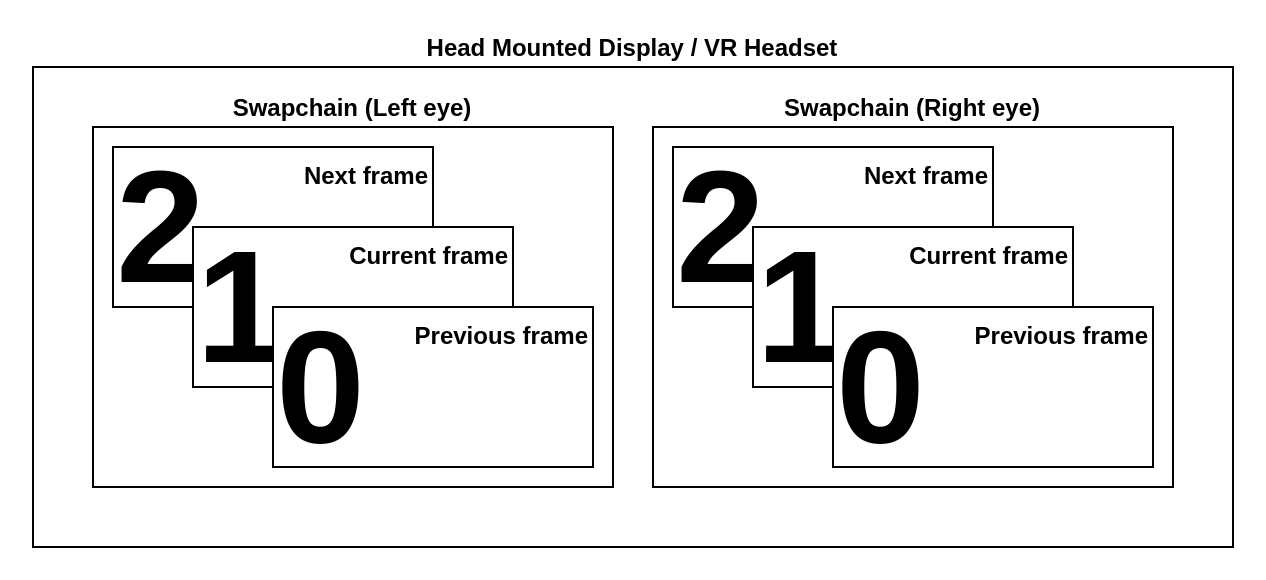
\includegraphics[scale=0.3]{resources/swapchains.png}
\end{figure}

Per comodità, all'interno del codice, è stata definita una struttura creativamente chiamata \texttt{Swapchain} la quale aiuta a semplificare il codice legando assieme i vari componenti di una swapchain: la lista delle immagini, la dimensione delle immagini e la struttura \texttt{XrSwapchain} di OpenXR.

Le swapchain vengono istanziate quando una sessione di OpenXR inizia, all'interno del metodo \texttt{bool begin\_session()}; una swapchain per view. Qui vengono create e configurate tutte le swapchain necessarie. Il metodo \texttt{shared\_ptr<Fbo> create\_fbo(GLuint w, GLuint h)} si occupa di generare le immagini (FBO = Frame Buffer Object) necessarie per le swapchain. Quest'ultimo fa affidamento alla classe \texttt{Fbo} già creata e utilizzata nel corso di realtà virtuale dal docente responsabile. Questa classe consiste in un wrapper attorno agli FBO di OpenGL e ne semplifica l'utilizzo. Grazie a questo, gli utenti avranno meno difficoltà quando dovranno utilizzare i framebuffer durante il rendering.

% TODO: https://registry.khronos.org/OpenXR/specs/1.0/man/html/XrViewConfigurationType.html
Il numero di swapchain è deciso in base alla \textit{view configuration type}. I due tipi di configurazione principali sono \textit{mono} e \textit{stereo}. Mono significa una singola view; questo è il caso per un'applicazione di realtà aumentata, dove l'unica view è presa dalla telecamera del dispositivo e gli oggetti virtuali vengono sovrapposti al mondo reale. Stereo, invece, indica due view. Questo è il caso di un visore di realtà virtuale da indossare (effettivamente degli occhiali) e richiede 2 view: una per l'occhio sinistro e una per l'occhio destro. XrBridge supporta solamente la configurazione stereo; è possibile però modificare il tipo di configurazione apportando poche e piccole modifiche. Questa configurazione è fatta all'inizio del metodo \texttt{bool begin\_session()}.

I framebuffer generati sono composti da una texture generata da OpenXR e il cui formato è specificato dall'utente (TODO: vedi capitolo Differenze fra piattaforme Windows e Linux) e un buffer di profondità.

\subsection{Spazio di riferimento}

In OpenXR, lo spazio di riferimento (\texttt{XrReferenceSpaceType}) è il sistema con cui un'applicazione VR tiene traccia della posizione e rotazione del mondo reale.

% TODO: Explain what type of reference space is used by default
Nel codice, lo spazio di riferimento è configurato durante la creazione di una sessione, alla fine del metodo \texttt{bool begin\_session()} dopo la creazione delle swapchain. Lo spazio di riferimento utilizzato può essere configurato attraverso la variabile \texttt{XRBRIDGE\_CONFIG\_SPACE} nella sezione di configurazione iniziale in \texttt{xrbridge.cpp}.

Di seguito sono riportati i principali spazi di riferimento disponibili in OpenXR senza fare uso di estensioni:

% TODO
\begin{table}[H]
  \caption{Tipi di spazi di riferimento}
  \begin{center}
    \begin{tabular}{ m{7cm} m{6cm} }
      Nome                                             & Descrizione \\
      \hline
      \texttt{XR\_REFERENCE\_SPACE\_TYPE\_VIEW}        & - \\
      \texttt{XR\_REFERENCE\_SPACE\_TYPE\_LOCAL}       & - \\
      \texttt{XR\_REFERENCE\_SPACE\_TYPE\_STAGE}       & - \\
      \texttt{XR\_REFERENCE\_SPACE\_TYPE\_LOCAL\_FLOOR} & Non disponibilie nella versione 1.0 di OpenXR. \\
    \end{tabular}
  \end{center}
\end{table}

% TODO: https://registry.khronos.org/OpenXR/specs/1.1/man/html/XrReferenceSpaceType.html
Per una descrizione più dettagliata, fare riferimento alla documentazione ufficiale.

\section{Limitazioni di FreeGLUT}

FreeGLUT è una libreria multi-piattaforma che permette di gestire finestre, contesti OpenGL, mouse e tastiera. L'utilizzo di questa libreria è obbligatoria dal momento che viene utilizzata dal corso di grafica e il corso di realtà virtuale. Per questo progetto, è stata utilizzata la versione 3.6.0.

% TODO: Mention why the teacher wants FreeGLUT and not other libraries

Come menzionato prima nel capitolo [Binding OpenGL + Linux], FreeGLUT non espone certi parametri che potrebbero essere necessari ad un'applicazione. È stato dunque necessario apportare modifiche alla libreria. Di seguito è descritto l'approccio scelto.

È stato aggiunto un nuovo file a FreeGLUT chiamato \texttt{freeglut\_globals.h} e, al suo interno, sono state definite due variabili globali:

\begin{verbatim}
  // Etratto da freeglut_globals.h
  uint32_t freeglut_visualid = 0;
  int freeglut_attributes[100] = { 0 };
\end{verbatim}

All'iterno di XrBridge, poi, includere questo file header e accedere alle variabili globali. Come parte della consegna del progetto, è anche presente una patch di git che descrive i cambiamenti effettuati nel dettaglio, così che possono essere facilmente applicati e analizzati.

\begin{quote}
  Attenzione! La versione modificata di FreeGLUT è stata verificata solamente su Linux; per utilizzare FreeGLUT su Windows, utilizzare la versione originale non modificata.
\end{quote}

Iniziando con il parametro più semplice: \texttt{visualid}. Questo si tratta di un semplice \texttt{uint32\_t}. È bastato aggiungere una singola riga di codice che assegna una il valore della variabile \texttt{visualInfo->visualid} alla variabile globale creata. Questo viene fatto all'interno della funzione \texttt{fgPlatformOpenWindow} nel file \texttt{src/x11/fg\_window\_x11.c}.

\begin{verbatim}
  // src/x11/fg_window_x11.c @ 432
  freeglut_visualid = visualInfo->visualid;
\end{verbatim}

Il secondo parametro è \texttt{glxFBConfig}. Questo è più complicato rispetto al precedente, pochè non si tratta di un semplice valore che può essere facilmente copiato, bensì di una struttura interna che non viene esposta all'utente se non attraverso un puntatore. Questa struttura viene generata dalla funzione \texttt{glXChooseFBConfig}, la quale accetta una serie di attributi assieme ad altri parametri e ritorna un puntatore ad una struttura di tipo \texttt{GLXFBConfig}. La soluzione è fortunatamente pittosto semplice: è sufficiente ottenere la lista di attributi usati per generare la struttura e invocare nuovamente il metodo \texttt{GLXFBConfig}. Per fare questo, è stato necessario salvare gli attributi in una delle variabili globali appena create. Questo è stato fatto nella funzione \texttt{fghChooseConfig} nel file \texttt{src/x11/fg\_window\_x11\_glx.c}. Infine, all'interno di XrBridge, è bastato chiamare la funzione \texttt{glXChooseFBConfig} con gli attributi corretti e così si ottiene la struttura necessaria.

\begin{verbatim}
  // src/x11/fg_window_x11_glx.c @ 102
  for (unsigned int i = 0; i < 100; ++i)
  {
    freeglut_attributes[i] = attributes[i];
  }
\end{verbatim}

Una libreria alternativa a FreeGLUT è GLFW, la quale espone i parametri interni attravero dei metodi specifici. Come menzionato all'inizio del capitolo, però, non è stato posibilie utilizzare questa libreria.

\section{Differenze fra piattaforme Windows e Linux}

Ci sono alcune importanti differenze fra le piattafrome Windows e Linux che hanno richiesto aggiustamenti all'interno del codice. In precedenza è già stato menzionato come il binding grafico differisce tra piattaforme (TODO: link to chapter); di seguito saranno presentate alcune differenze che hanno causato difficoltà nello sviluppo di XrBridge.

Quando si tratta di generare i framebuffers per ogni view/occhio, è possibile specificare il formato dell'immagine desiderato (es: GL\_RGBA16F, GL\_SRGB8, ...). Il formato dipende fortemente dalla API grafica scelta e la runtime, dal momento che OpenXR non specifica alcun formato di default.

Una delle difficoltà riscontrate durante lo sviluppo, è il fatto che SteamVR supporta formati diversi a seconda della piattaforma. Di seguito sono elencati alcuni dei formati supportati da SteamVR sulle piattaforme principali dalla versione attuale di SteamVR (2.7.4 su Windows e Linux; non sono state verificate le versioni beta):

\begin{table}[H]
  \caption{Formati immagine di OpenGL supportati da SteamVR}
  \begin{center}
    \begin{tabular}{ l l l }
      Formato                    & Windows & Linux \\
      \hline
      \texttt{GL\_RGB8}          & No      & No    \\
      \texttt{GL\_RGB16}         & No      & No    \\
      \texttt{GL\_RGBA8}         & No      & No    \\
      \texttt{GL\_RGBA16}        & Sì      & No    \\
      \texttt{GL\_RGB8\_SNORM}   & No      & No    \\
      \texttt{GL\_RGB16\_SNORM}  & No      & No    \\
      \texttt{GL\_RGBA8\_SNORM}  & No      & No    \\
      \texttt{GL\_RGBA16\_SNORM} & No      & No    \\
      \texttt{GL\_RGB16F}        & Sì      & No    \\
      \texttt{GL\_RGB32F}        & No      & No    \\
      \texttt{GL\_RGBA16F}       & Sì      & No    \\
      \texttt{GL\_RGBA32F}       & No      & No    \\
      \texttt{GL\_RGB8I}         & No      & No    \\
      \texttt{GL\_RGB16I}        & No      & No    \\
      \texttt{GL\_RGB32I}        & No      & No    \\
      \texttt{GL\_RGB8UI}        & No      & No    \\
      \texttt{GL\_RGB16UI}       & No      & No    \\
      \texttt{GL\_RGB32UI}       & No      & No    \\
      \texttt{GL\_RGBA8I}        & No      & No    \\
      \texttt{GL\_RGBA16I}       & No      & No    \\
      \texttt{GL\_RGBA32I}       & No      & No    \\
      \texttt{GL\_RGBA8UI}       & No      & No    \\
      \texttt{GL\_RGBA16UI}      & No      & No    \\
      \texttt{GL\_RGBA32UI}      & No      & No    \\
      \texttt{GL\_SRGB8}         & Sì      & Sì    \\
      \texttt{GL\_SRGB8\_ALPHA8} & Sì      & Sì    \\
      \texttt{GL\_RGB9\_E5}      & No      & No    \\
    \end{tabular}
  \end{center}
\end{table}

SteamVR è costantemente aggiornato e, perciò, è molto probabile che in futuro i formati supportati cambino.

Scegliere un formato non supportato causerà l'errore \texttt{XR\_ERROR\_SWAPCHAIN\_FORMAT\_UNSUPPORTED} (-26).

A causa di queste differenze, è stato deciso di permettere all'utente di specificare il formato per piattaforma invece di avere una singola configurazione globale.

Nella sezione di configurazione di XrBridge (all'inizio del file \texttt{xrbridge.cpp}) è possibile specificare il formato con le variabili \texttt{XRBRIDGE\_CONFIG\_SWAPCHAIN\_FORMAT\_WINDOWS} e \texttt{XRBRIDGE\_CONFIG\_SWAPCHAIN\_FORMAT\_LINUX}.

\section{Strumenti, librerie e versioni}

Di seguito sono riportate le versioni di tutti gli strumenti, software e librerie utilizzate per il progetto. Non sono necessariamente richieste le stesse identiche versioni per eseguire l'applicazione di demo o per utilizzare XrBridge.

% TODO: Check versions on actual Linux dev system
\begin{table}[H]
  \caption{Versioni di strumenti e librerie utilizzati}
  \begin{center}
    \begin{tabular}{ m{4cm} m{2cm} m{7cm} }
      Strumento & Versione & Note \\
      \hline
      ALVR & 20.8.0 & Software per Windows e Linux che permette di utilizzare un dispositivo Android come un headset. \\
      PhoneVR & 2.0.0 & Software per Android che permette di utilizzare un dispositivo Android come un headset. \\
      SteamVR & 2.7.4 & Runtime di OpenXR sviluppata da Valve. \\
      Visual Studio Community 2022 & 17.11.1 & IDE per sviluppare su Windows. \\
      Code::Blocks & svn-r13524 & IDE per sviluppare su Linux. \\
      Windows 11 & TODO & Piattaforma di sviluppo Windows. \\
      Fedora 40 KDE & 6.10.6 & Piattaforma di sviluppo Linux. \\
      OpenXR & 1.0.0 & Versione di OpenXR utilizzata per sviluppare XrBridge. \\
      FreeGLUT & 3.6.0 & Libreria di supporto per OpenGL (utilizzata sia su Windows sia per la versione modificata per Linux). \\
      GLEW & 2.1.0 & Libreria di supporto per OpenGL (Windows). \\
      GLEW (glew) & 2.2.0 & Libreria di supporto per OpenGL (Linux). \\
      GLM & 1.0.1 & Libreria matematica per OpenGL (Windows).\\
      GLM (glm-devel) & 0.9.9 & Libreria matematica per OpenGL (Linux). \\
      OpenXR Loader & 1.1.37 & Loader per OpenXR (Windows, compilato manualmente). \\
      OpenXR Loader (openxr, openxr-devel) & 1.0.33 & Loader per OpenXR (Linux). \\
      Nvidia GTX 970 & & GPU utilizzata. \\
      Nvidia & 555.58.03 & Driver video per Nvidia. \\
    \end{tabular}
  \end{center}
\end{table}

\chapter{Risultati}

% TODO: Talk about what requirements have been completed

\section{Manuale d'uso}

Di seguito verrà spiegato nel dettaglio come utilizzare XrBridge in un progetto reale. Nel caso di difficoltà, è possibile utilizzare l'applicazione di demo come base per lo sviluppo. L'applicazione di demo ha un progetto per Visual Studio 2022 e Code::Blocks. Questa sezione è principalmente mirata al docente responsabile.

\subsection{Dipendenze}

XrBridge fa uso delle seguenti dipendenze \textbf{obbligatorie}:

% TODO: Define C++ version
\begin{itemize}
  \item \textbf{Libreria standard di C++}: XrBridge utilizza alcune funzionalità dalla libreria standard di C++. È sufficiente assicurarsi di utilizzare un'implementazione completa di C++ XX (TODO:Version).
  \item \textbf{GLM}: GLM si tratta di una libreria matematica per facilitare lo sviluppo con OpenGL. XrBridge fa uso di questa libreria per calcolare le matrici di view e proiezione da utilizzare per il rendering.
  \item \textbf{GLEW}: GLEW è una libreria che permette di utilizzare funzionalità più avanzate di OpenGL.
  \item \textbf{FreeGLUT}: FreeGLUT è una libreria che permette di creare finestre, ricevere input e gestire contesti di OpenGL. Questa libreria si occupa di creare il contesto di OpenGL, dal quale sono necessari alcuni parametri importanti.
  \item \textbf{Fbo}: XrBridge fa affidamento alla classe \texttt{Fbo} sviluppata dal docente responabile per facilitare la gestione dei framebuffers di OpenGL.
  \item \textbf{OpenXR}: XrBridge è stato sviluppato basandosi sulla versione di OpenXR 1.0.0 per permettere una maggiore compatibilità. È possibilie utilizzare versioni più recenti se desiderato.
  \item \textbf{Win32}: Per Windows, è necessario acesso alla API di Windows (\texttt{Windows.h}). Questa libreria dovrebbe esere già presente.
  \item \textbf{Xlib}: Per Linux, è necessaria la libreria Xlib per interagire con X11. Per utilizzare XrBridge su Wayland, è possibile utilizzare XWayland.
\end{itemize}

% TODO: Reference version table
Per quanto riguarda le versioni delle librerie, fare riferimento alla tabella apposita. Notare che non è sempre necessario avere la verione esatta di una libreria.

Per quanto riguarda Windows, sono già fornite tutte le dipendenze necesarie assieme all'applicazione di demo. È possibile utilizzare le librerie fornite.

% TODO: Reference version table
Su Linux, invece, è possibile utilizzare il package manager della distribuzione scelta. Per questo progetto, è stato utilizzato DNF, parte di Fedora 40. Nella tabella delle versioni è specificato il nome del pacchetto su Fedora.

\subsection{Setup del progetto}

È possibile utilizzare qualsiasi IDE per sviluppare un'appicazione con XrBridge; oppure nessuna. Per sviluppare l'applicazione di demo su Windows è stato utilizzato Visual Studio e Code::Blocks su Linux.

Il primo passo è creare un progetto e importare XrBridge. È sufficiente copiare i file \texttt{xrbridge.cpp}, \texttt{xrbridge.hpp}, \texttt{fbo.cpp} e \texttt{fbo.h} all'interno del progetto.

Il compilatore genererà reclamerà per la mancanza delle dipendenze. A questo punto aggiungere le ipendenze necessarie (FreeGLUT, GLFW, OpenXR, GLM, ...). È importante ricordarsi che su Linux è necessario utilizzare la versione modificata di FreeGLUT.

Se si utilizza Visual Studio, è possibile incontrare un errore relativo all'uso della funzione non sicura \texttt{std::strncpy}. Per risolvere questo problema, definire a la macro \texttt{\_CRT\_SECURE\_NO\_WARNINGS} a livello di progetto (non necessita di nessun valore, è sufficiente che sia definita). In alternativa, aggiungere \texttt{\#define \_CRT\_SECURE\_NO\_WARNINGS} all'inizio del file \texttt{xrbridge.cpp}.

Se si desidera attivare l'output di debug è sufficiente definire la macro \texttt{XRBRIDGE\_DEBUG} a livello di progetto.

Come ultima cosa è necessario scegliere la piattaforma da utilizzare. Per compilare XrBridge con supporto per Winows, definire la macro \texttt{XRBRIDGE\_PLATFORM\_WINDOWS}, mentre definire \texttt{XRBRIDGE\_PLATFORM\_X11} per Linux. Anche queste macro sono da definire a livello di progetto. XrBridge non si compila se una macro non viene definita; si genererà un errore che menziona come \texttt{graphics\_binding} non è stato definito.

\subsection{Codice}

Per poter accedere alle funzionalità di XrBridge nel codice, è necessario includere il file appropriato:

\begin{verbatim}
  #include "xrbridge.hpp"
\end{verbatim}

Questo darà accesso alla classe \texttt{XrBridge}. Tutte le funzionalità necessarie sono contenute qui.

È fondamentale inizializzare il FreeGLUT e il contesto OpenGL \textbf{prima} di utilizzare XrBridge!

In seguito, si crea un'istanza di XrBridge e la si inizializza:

\begin{verbatim}
  XrBridge xrbridge;
  if (xrbridge.init("XrBridge Demo") == false)
  {
    // Error handling ...
  }
\end{verbatim}

Nel caso l'inizializzazione fallisca, l'oggetto XrBridge non sarà utilizzabile. Un fallimento in questo caso è probabilmente dovuto ad un errore di configurazione dell'ambiente dell'utente. Analizzare l'errore riportato a terminale, risolvere il problema e riprovare.

La stringa passata al metodo \texttt{init} non è di molta importanza. Nel caso di SteamVR, questa sarà usata come titolo dell'applicazione che verrà mostrata a schermo e non influisce sull'esecuzione dell'applicazione.

Opzionalmente, configurare i clipping planes che verranno utilizzati per generare le matrici di proiezione. Questo passo può essere eseguito in qualunque momento e per quante volte si desidera (fare questo durante il render potrebbe creare artefatti grafici indesiderati):

\begin{verbatim}
  xrbridge.set_clipping_planes(0.1f, 65'536.0f);
\end{verbatim}

% TODO

Per ultimo, ricordarsi di liberare tutte le risorse utilizzate:

\begin{verbatim}
  xrbridge.free();
\end{verbatim}

Dopo questo, l'istanza di XrBridge non sarà più utilizzabile. Riavviare l'applicazione o creare una nuova istanza se desiderato.

\begin{quote}
  Attenzione! Questo passo va eseguito \textbf{prima} di eliminare il contesto OpenGL!
\end{quote}


\subsection{Runtime}

\section{XrBridge vs OvVR}

% TODO: Compare XrBridge to OvVR with example code

\section{Test}

\chapter{Conclusioni}

\lipsum[23]
Esempio di citazione \cite{4538384}, \cite{5357331,4523385}, \cite{1705631}.
\footnote{Questa \`e una nota a pi\'e di pagina.}
\footnote{Questa \`e un'altra nota a pi\'e di pagina.}

\bibliographystyle{unsrt}
\bibliography{bibliografia}

\end{document}
